% 手拉手 例2：两个等腰直角三角形共顶点 O，∠AOB=∠COD=90°，AC⊥BD
\documentclass[tikz,border=4pt]{standalone}
\usepackage{ctex}
\usepackage{amsmath}
\usetikzlibrary{calc, decorations.markings}
\begin{document}
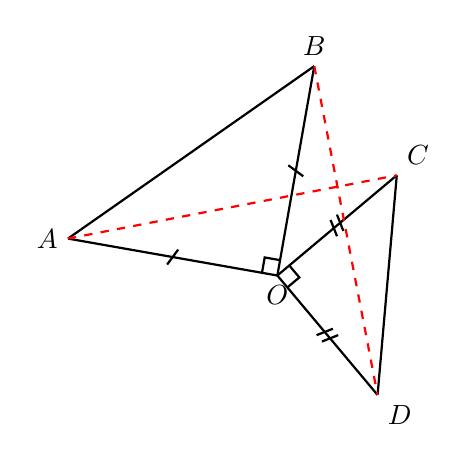
\begin{tikzpicture}[scale=0.9, thick,
  tick/.style={postaction={decorate, decoration={markings,
    mark=at position 0.5 with {\draw (-1.5pt,-3pt) -- (1.5pt,3pt);}}}},
  ticktwo/.style={postaction={decorate, decoration={markings,
    mark=at position 0.5 with {\draw (-2.5pt,-3pt) -- (-0.5pt,3pt);
                               \draw (0.5pt,-3pt)  -- (2.5pt,3pt);}}}}]
  \coordinate (O) at (0,0);
  % △OAB 顶角 90°，OA=OB=3，A 在 170°, B 在 80°
  \coordinate (A) at ({3*cos(170)}, {3*sin(170)});
  \coordinate (B) at ({3*cos(80)}, {3*sin(80)});
  % △OCD 顶角 90°，OC=OD=2.2，C 在 40°, D 在 -50°
  \coordinate (C) at ({2.2*cos(40)}, {2.2*sin(40)});
  \coordinate (D) at ({2.2*cos(-50)}, {2.2*sin(-50)});

  \draw[tick] (O) -- (A);
  \draw[tick] (O) -- (B);
  \draw (A) -- (B);
  \draw[ticktwo] (O) -- (C);
  \draw[ticktwo] (O) -- (D);
  \draw (C) -- (D);

  % 直角小方块
  \draw ($(O)+(170:0.22)$) -- ($(O)+(170:0.22)+(80:0.22)$) -- ($(O)+(80:0.22)$);
  \draw ($(O)+(40:0.22)$) -- ($(O)+(40:0.22)+(-50:0.22)$) -- ($(O)+(-50:0.22)$);

  \draw[red, dashed] (A) -- (C);
  \draw[red, dashed] (B) -- (D);

  \node[below]       at (O) {$O$};
  \node[left]        at (A) {$A$};
  \node[above]       at (B) {$B$};
  \node[above right] at (C) {$C$};
  \node[below right] at (D) {$D$};
\end{tikzpicture}
\end{document}
